\documentclass[11pt,oneside,final,letterpaper]{memoir}
%%%%%%%%%%%%%%%%%%%%%%%%%%%%%%%%%%%%%%%%%%%%%%%%%%%%%%%%%%%%%%%%%%%%%%%%%%%%%%%%
% packages | mi-laser-doc.tex
%%%%%%%%%%%%%%%%%%%%%%%%%%%%%%%%%%%%%%%%%%%%%%%%%%%%%%%%%%%%%%%%%%%%%%%%%%%%%%%%

% graphics
\usepackage{graphicx}  % graphics
\usepackage{epstopdf}  % eps files
\graphicspath{{../Images/}}  % images location

% layout
\usepackage{float}     % forced figure positioning
\usepackage{caption}   % caption formatting
\captionsetup[figure]{labelfont=bf,width=1.00\textwidth} %figure captions
\captionsetup[table]{labelfont=bf,width=1.00\textwidth}  %table captions
\captionsetup{font=small}

% text
\usepackage{lmodern}   % latin modern fonts, for palatino
\usepackage{booktabs}  % booktabs for perfect tables
\usepackage{lipsum}    % for blind text
\usepackage{amsmath}   % ams math environments and commands
\usepackage{textcomp}  % more math stuff
\usepackage{tikz}      % this is a graphics package but we will use it to print page #
\usepackage{pxfonts}   % package for palatino support
\usepackage{tgpagella} % package for palatino support (math mode)
\usepackage{hyperref}  % links

% bonus colors
\usepackage{xcolor}

% osa blue = 47/255, 66/255, 154/255
\definecolor{OSABlue}{rgb}{0.1845, .259, 0.604}

% color chapter names
\renewcommand\chapnumfont{%
    \leavevmode\Huge\bfseries\color{OSABlue}\sffamily%
}%
\renewcommand\chapnamefont{%
    \leavevmode\Huge\bfseries\color{OSABlue}\sffamily%
}%
\renewcommand\chaptitlefont{%
    \leavevmode\Huge\bfseries\color{OSABlue}\sffamily%
}%
\setsecheadstyle{%
    \leavevmode\Large\bfseries\color{OSABlue}\sffamily%
}%

% finesee table and figure numbering
\renewcommand{\thefigure}{%
    \arabic{figure}
}
\renewcommand{\thetable}{%
    \arabic{table}
}
% table of contents depth
\maxtocdepth{subsection}

% stretching row height in tables
\newcommand{\ra}[1]{\renewcommand{\arraystretch}{#1}} % ex: \ra{1.2}

% the iron rule of palatino
\renewcommand{\rmdefault}{ppl}

% links
\hypersetup{
    colorlinks=true,
    linkcolor=black,
    citecolor=[rgb]{0.0078,0.2431,0.9725},
    urlcolor=[rgb]{0.0078,0.2431,0.9725}
}

\title{The Design and Fabrication of a Laser Obstacle Course}
\author{Brandon Dube, David Lippman, Kai Williams, JT Pirog}
\date{November 3, 2016}
\begin{document}

\begin{titlingpage}
\begin{center}
    \includegraphics[width=1.0\textwidth]{StudentChapterLogo} \\
    \vspace*{10pt}
    \textsf{
        \textbf{%
            \Huge{%
                \textcolor{OSABlue}{%
                    The Design and Fabrication of a Laser Obstacle Course
                }
            }
        } \\
        \vspace*{12pt}
        \large{Brandon Dube\textsuperscript{1}, David Lippman, Kai Williams, JT Pirog \\}
        \small{\textsuperscript{1}\hspace*{-0.25em} Corresponding author: \href{mailto:bdube@u.rochester.edu}{bdube@u.rochester.edu}} \\
        \vspace*{24pt}
        \Large\textbf{\textcolor{OSABlue}{Abstract}} \\
    }
\end{center}

\noindent In this document we describe the construction and operation of a laser obstacle course, the outreach activity of the century.  The course is 12$\times{}$8' in size and uses 10 lasers in order to provide a challenging player experience.  It features an upward-counting clock as well as leaderboard on separate displays as well as a built in sound system.  It is driven by the Raspberry Pi and Arduino low cost computing platforms available today.

\vspace*{\fill}
\noindent\small{%
Thanks to Raymond Lopez-Rios, Jaren Ashcraft, and Aizhong Zhang for their help realizing this project.\\ \\
Thanks also to The Optical Society, the Special Programs grant received made this effort possible.
}
\end{titlingpage}

\chapter*{Introduction}
   
Many action movies feature some sort of laser security system like the one seen below in \textit{Ocean's Twelve (2004)}.  They are a hallmark of the genre and often some of the most memorable scenes in the films.  We have sought to recreate these devices, albeit on a smaller scale and with less grand scenery.  Our lasers are also red and not blue.  Commercial versions of this attraction exist, often in laser tag venues and special effects museums.  These are prohibitively expensive to frequent, and require transport to get players to the course.  This creates a barrier to access.

We have brought the course to the players while providing an engineering project experience for members of our organization.  Many optical devices are used in these defense systems (or obstacle courses, as it were); in this way the device can also serve as an outreach activity.

We hope that this document can serve not only as a reference for what we have ultimately done, but also provide some information about portions of this project that were not successful.

\vspace*{\fill}
\begin{center}
\includegraphics[width=1.0\textwidth]{O12-Intro-brightened-compressed}
\end{center}

%\par\smallskip\noindent\centerline{
%    \begin{minipage}{1.25\textwidth}
%        \begin{center}
%            \includegraphics[width=1.0\textwidth]{O12-Intro-brightened-compressed}
%        \end{center}
%    \end{minipage}
%}

\chapter*{Concept}

Because the creators of this course will not be at the university forever, it was important to us that the course be as simple to operate as possible.  It is also likely to suffer a few drops over its lifetime, so it should be robust.  Our organization does not have unlimited funding, so it should also be relatively low cost.

With these criteria in mind, we set out to design and build our dream, turning it into a reality.

%\chapter*{Hardware}
%\chapter*{Optics}
%\chapter*{Optomechanics}
\chapter*{Electronics}

In keeping with the low cost requirement of the project, we forewent complex systems for the electrical components of this project.  There are no ``full-scale'' computers, no specialized hardware, no multiplexing and no complex circuits.  The game only requires that we be able to read signals and respond to changes in them, drive two displays, and power ten lasers.  Complicated custom hardware can be developed to do this with microcontrollers and microprocessors, but most of the legwork has already been done in that area.  The Arduino platform uses low power 16MHz microcontrollers with tiny (by today's standards) amounts of memory and a large number of raw I/O pins to enable amateur makers to produce electronics that talk to the real world with ease.  Despite the extremely low power, an Arduino is actually capable of running a program that handles all aspects of this game, more power is only needed for audio playback and display.

For these actions, we expand to the Raspberry Pi platform.  The Pi is a low-cost \textsc{arm} based computer that features 40 pins of I/O that allow it to talk to electrical devices, in addition to an ethernet port, \textsc{hdmi} port, SD card slot, and other normal computer hardware.  Its much faster 1.2Ghz quad-core processor allows it to do heavy lifting far beyond what an Arduino is capable of.  The Raspberry Pi is used to drive the displays and perform computations.  An Arduino Mega serves as an input analog to digital converter (\textsc{adc}).

\section*{System Design}

Here we outline the laser course's electronics on a system level.  We provide a block diagram, as well as the circuit design of each component.  A 12V 5A \textsc{ac-dc} power supply is used to provide the power for all components of the system.  Power supplies at 8V, 5V, and 3.3V are fed off of its output.

\begin{figure}[H]
    \rotatebox{90}{
        \begin{minipage}{\textheight}
            \includegraphics[width=1.0\linewidth]{System_schem}
        \end{minipage}}
        \caption[The schematic view of the entire system.]{
            The schematic view of the electrical system as a whole.  This drawing is missing 9 photoresistors and 9 laser diodes, as well as the adjust and output resistors on the voltage regulators.  It will be updated at a later date.  The state and end buttons signal the Arduino, which in turn can alter the state of the relay and transmit data to the Pi, which performs the necessary calculations and drives the display.
        }
\end{figure}

\autoref{fig:ACDCPowerSupply_schem} is a generic \textsc{ac-dc} power supply circuit.  The voltage is stepped down through a transformer, its - oscillation is removed with a bridge rectifier, then the output is stabilized and made constant by buffering through capacitors.  Finally, a linear voltage regulator is placed at the end of the supply and slightly reduces the voltage in order to provide a safe output.  The capacitors have a nice side effect of allowing the supply to provide much higher peak current than its continuous current rating.  A 5A power supply may be capable of 50A peak output for short periods on the order of milliseconds.

\begin{figure}[H]
    \centering
    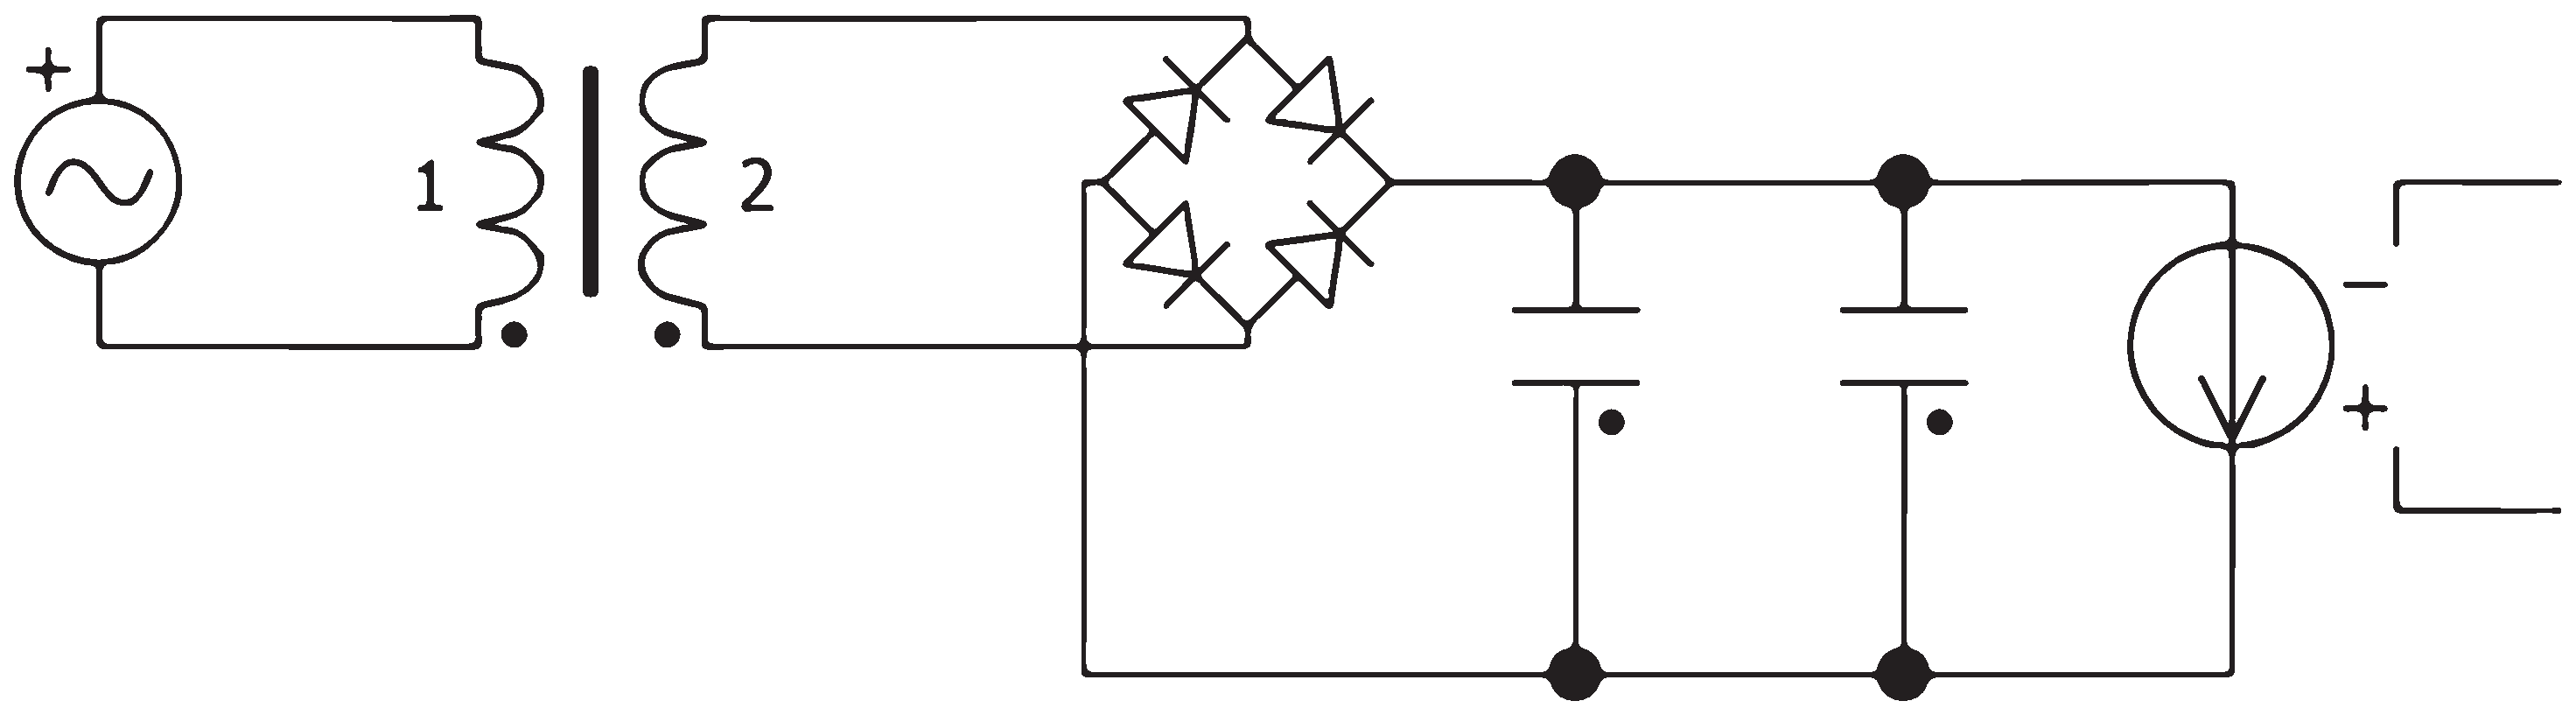
\includegraphics[width=1.0\textwidth]{AC_DC_power_supply}
    \caption[Generic AC-DC power supply]{
        A generic \textsc{ac} to \textsc{dc} power supply.  \textsc{ac} voltage at line level enters and is passed into a transformer that reduces the voltage to one moderately higher than the desired output voltage.  A Bridge Rectifier converts the AC current into DC current, the power is double filtered through capacitors to remove the oscillations, and a linear regulator provides stable \textsc{dc} power at the desired output voltage.
    } \label{fig:ACDCPowerSupply_schem}
\end{figure}

This \textsc{ac-dc} supply serves as the input state to our power supply network.  A set of LM317 Linear Voltage Regulators from OmSemi or Texas Instruments (both produce the same part) are used to form \textsc{dc-dc} power supplies with voltages set to 8V, 5V, and 3.3V.  The 8V supply feeds the Arduino while the 5V supply serves as the \textsc{vcc} for the photoresistor circuits and switches and powers the Pi.  The 3.3V supply powers the lasers.

\begin{figure}[H]
    \centering
    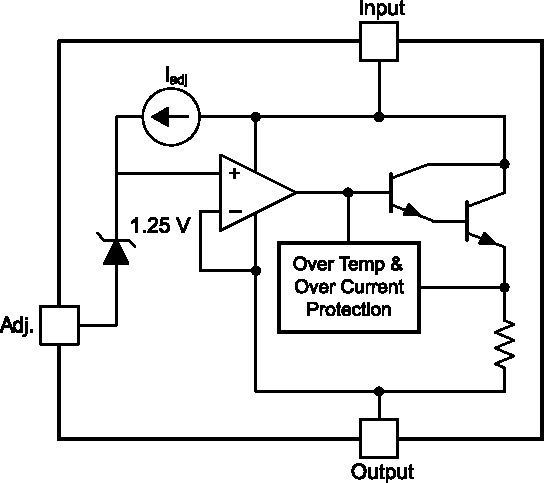
\includegraphics[width=4.5in]{lm317}
    \caption[Texas Instruments LM317 Block Diagram]{
        The block diagram of the LM317 as provided by Texas Instruments.
    } \label{fig:LM317_schem}
\end{figure}

The output voltage of these devices is tunable to be anything from 1.2-40V depending on the resistors connected between its pins.  It is also constrained to be less than 80\% of the input voltage.  The resistors do not carry current, and serve to bias the circuit inside of the regulator. \autoref{eq:LM317Resistors} is used to compute the resistor values needed to produce a given output voltage.  In use, one specifies $V_{Out}$ and chooses one resistor value arbitrarily to solve for the other resistor needed.

\begin{equation} \label{eq:LM317Resistors}
R_2 = R_1 \left( \frac{V_{\text{Out}}}{1.25} - 1\right)
\end{equation}

The 8V output of the first LM317 powers the Arduino and is used as the input stage to another LM317, which produces a 5V output which is used as a high-current \textsc{vcc} supply for the photoresistor circuits.  The 5V output is used as the input to create a 3.3V supply, which is used to power the lasers.  Driven at 3.3V, they output about 0.85mW of power.

\section*{Optoelectronic Circuits}

We use the Arduino's 5V bus as a \textsc{vcc} or reference voltage output and ground pins to create a low-current power supply.  From this we create one circuit for each photoresistor.  These circuits are very simply.  The positive \textsc{vcc} voltage is passed over one terminal of the resistor.  At the other terminal there are two connections in parallel.  A regular resistor connects the circuit to ground; this is known as a pull-down resistor, and its job is to prevent the output voltage of this circuit from floating between 0 and \textsc{vcc}.  The other connection is a simple lead to an analog input pin of the Arduino.  Ten of these circuits are present on the custom PCB that has been purchased for the project, with one lead to the Arduino for each its 5V output (\textsc{vcc}) and ground pins, and one ``reading'' lead for each photoresistor.  Each circuit presents a voltage between 5V (0 $\Omega$) and 0V ($\infty \, \Omega$) depending on the value of the photoresistor.  Each analog input pin will produce a value between 0 and 1023 depending on the input voltage.

The Arduino also signals the control pins of a relay (an electrically toggle-able switch) that cycles the lasers on and off.  While the continuous draw of the lasers (\textless\thinspace 2mA) is below the 40mW output capacity of the addressable pins of the Arduino, the current draw as they turn on can be much higher, up to approximately 300mA.  This phenomenon is known as inrush current and is shown in \autoref{fig:InrushCurrent}.  Pulsing the lasers for effect risks burning out the Arduino's pins.  By providing an external power supply and opening and closing its circuit remotely, there is no risk to the Arduino.  The relay's much greater heat dissipation allows it to handle the inrush current with ease, and the power supply used is capable of providing over 20 amps of long-term current at 3.3V.

\begin{figure}[H]
    \centering
    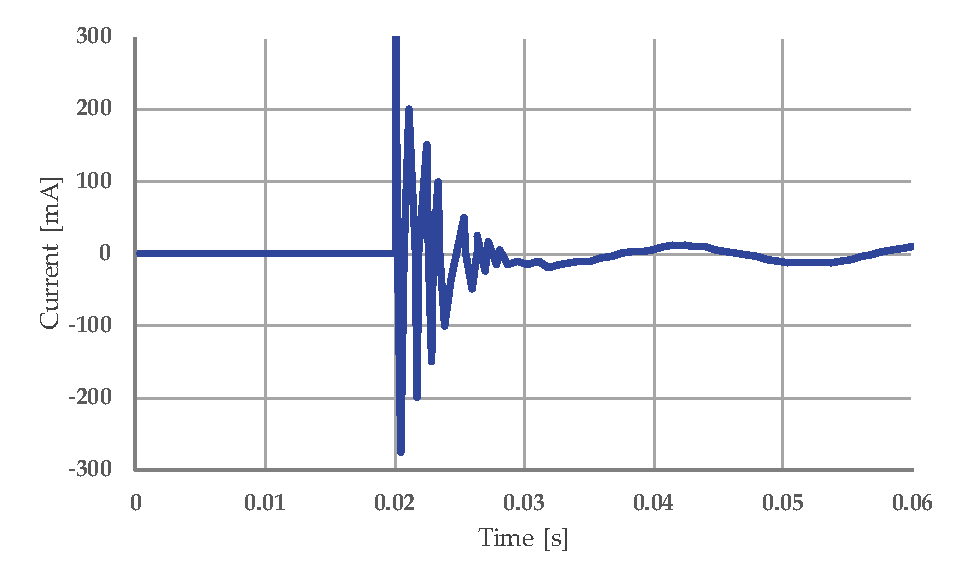
\includegraphics[width=1.0\textwidth]{Inrush_current}
    \caption[Oscilloscope measurement of inrush current]{
        An oscilloscope measurement of the inrush current of a diode-pumped laser.  The current draw eventually stabilizes to 1mA, but can reach values of up to 300mA for a short time.  If the laser is pulsed at 24Hz, the initial behavior is repeated so frequently that the time average current is about 25mA - over ten times higher than the continuous or long-term current draw.
    } \label{fig:InrushCurrent}
\end{figure}

\begin{figure}[H]
    \centering
    \includegraphics[width=1.0\textwidth]{Mega-Photoresistor_bb}
    \caption[Arduino and Photoresistor on a Breadboard]{
        The Arduino Mega and a single photoresistor circuit on a breadboard.  The 5V power supply on the Arduino provides the reference voltage, which is passed over the photoresistor.  In this case, a 220$\Omega{}$ resistor is used as the pulldown resistor that prevents the voltage from floating.  This is in series \textbf{before} the connection to the analog input pin that will read the voltage.
    } \label{fig:ArduinoPhotoresistor_bb}
\end{figure}

\begin{figure}[H]
    \centering
    \includegraphics[width=1.0\textwidth]{Mega-Photoresistor_schem}
    \caption[Arduino and Photoresistor Schematic]{
        The schematic view of the same circuit seen in \autoref{fig:ArduinoPhotoresistor_bb}.
    } \label{fig:ArduinoPhotoresistor_schem}
\end{figure}

\begin{figure}[H]
    \rotatebox{90}{
        \begin{minipage}{\textheight}
            \includegraphics[width=1.0\linewidth]{ArduinoIO_schem}
        \end{minipage}}
        \caption[The schematic view of 10 photoresistor circuits wired to the Arduino Mega.]{
            The schematic view of 10 photoresistor circuits wired to the Arduino Mega.  Each photoresistor-resistor circuit is in parallel along a +5V rail and a \textsc{gnd} rail.  The I/O to the Raspberry Pi and relay is also shown.
        }
\end{figure}

\section*{Communication}

Because we are utilizing multiple low-power compute platforms, we must establish a protocol of communication between them.  Both the Arduino and Pi support serial communication which provides us the ability to send complex signals between the two quickly over a single pin.  These signals must be encoded and decoded on each platform.  Here, we outline the chatter between the Arduino and Pi.

The Arduino communicates the state of the game's physical components to the Pi over a serial connection.  It is capable of reading all of its pins very quickly (thousands of times per second), faster than the Pi can process its serial input.  To solve this issue, we implement a clock and send signals at a fixed rate of 24Hz for a cinematic experience.  Each communication is encoded as \texttt{laserState-pr01-pr02-pr03...-pr10} where \texttt{laserState} is a 1 for on, 0 for off.  pr01 -- pr10 are the digital values for the voltage reading from each photoresistor and takes values between 0000 and 1023.  An example communication may be the following if all of the photoresistors have been burnt up and gone to zero resistance:

\begin{center}
\texttt{1-1023-1023-1023-1023-1023-1023-1023-1023-1023-1023}
\end{center}

The Arduino also reads a reply from the Pi after each communication.  These replies are similarly encoded, and command the Arduino to turn the lasers on or off, pulse them, and so forth.

%\chapter*{Setup}
%\chapter*{Operation}

\chapter*{Safety Features and Testing}

This project has been safety tested for most of its features.  There is a risk of collapse of the panels upon the players, electrical shock, and eye damage from the lasers.  

The lasers have been tested by connecting a sample assembly to a lab power supply.  The supply was set to 3.3V DC and an optical power meter was used to measure the power output of the laser.  The power was found to be \textcolor{red}{0.85mW}.  The LM317 fed power supply in the course' circuit is configured for a 3.28V output which has been verified with a multimeter.  All 10 lasers are wired in parallel and receive the same voltage.

This power output conforms to Class II laser specifications and is considered eye safe.

\vspace*{\fill}
\begin{flushright}
last updated 2016.10.30
\end{flushright}
\end{document}